%!TEX program = pdflatex
%----------------------------------------------------------------------------------------
% TEMPLATE INFORMATON
%----------------------------------------------------------------------------------------
% This template was adapted from "The Legrand Orange Book Version 1.4 (12/4/14) [http://www.LaTeXTemplates.com] Mathias Legrand (legrand.mathias@gmail.com)" License: CC BY-NC-SA 3.0 (http://creativecommons.org/licenses/by-nc-sa/3.0/)
%----------------------------------------------------------------------------------------

%----------------------------------------------------------------------------------------
% COMPILACAO
%----------------------------------------------------------------------------------------
% 0) There is a "compilar.sh"
% OR
% 1) pdflatex livro_algoritmos_e_estruturas_de_dados
% 2) makeindex livro_algoritmos_e_estruturas_de_dados.idx -s StyleInd.ist
% 3) biber livro_algoritmos_e_estruturas_de_dados
% 4) pdflatex livro_algoritmos_e_estruturas_de_dados
% 5) pdflatex livro_algoritmos_e_estruturas_de_dados

%----------------------------------------------------------------------------------------
%	PACKAGES AND OTHER DOCUMENT CONFIGURATIONS
%----------------------------------------------------------------------------------------
\documentclass[11pt,fleqn]{book} % Default font size and left-justified equations

%encoding
%--------------------------------------
\usepackage[T1]{fontenc}
%--------------------------------------
\usepackage[utf8]{inputenc}
\hyphenation{Mi-nis-té-ri-o}
\hyphenation{des-pre-za-das}
\usepackage[top=3cm,bottom=3cm,left=3.2cm,right=3.2cm,headsep=10pt,a4paper]{geometry} % Page margins
\usepackage[svgnames]{xcolor} % Required for specifying colors by name
\definecolor{blue}{rgb}{0.0, 0.18, 0.39}
% Font Settings
\usepackage{avant} % Use the Avantgarde font for headings
%\usepackage{times} % Use the Times font for headings
\usepackage{mathptmx} % Use the Adobe Times Roman as the default text font together with math symbols from the Sym­bol, Chancery and Com­puter Modern fonts
\usepackage{microtype} % Slightly tweak font spacing for aesthetics
% Index
\usepackage{calc} % For simpler calculation - used for spacing the index letter headings correctly
\usepackage{makeidx} % Required to make an indexs
\makeindex % Tells LaTeX to create the files required for indexing
\usepackage{verbatim}
% Others
\definecolor{lightGray}{gray}{0.95}
\usepackage[
colorinlistoftodos, 
prependcaption, 
color=green,
textsize=small, 
linecolor=red, 
backgroundcolor=lightGray, 
bordercolor=black]{todonotes}
\usepackage{epigraph}
\renewcommand{\textflush}{flushepinormal}
\setlength{\epigraphwidth}{0.8\textwidth}

\usepackage{nameref}
\usepackage{booktabs}
\usepackage{graphicx}
\usepackage{float}
\usepackage{multirow}

%CODE
\usepackage{courier}
\usepackage{listings}
\usepackage{courier}
\lstset{
	numbers=left,                   % where to put the line-numbers
	stepnumber=1,                   % the step between two line-numbers. 	
	frame=tb,                       % draw a frame at the top and bottom of the code block
	tabsize=4,                      % tab space width
	showstringspaces=false,         % don't mark spaces in strings
	numbers=left,                   % display line numbers on the left
	commentstyle=\color{Gray},      % comment color
	keywordstyle=\color{DarkBlue},  % keyword color
	stringstyle=\color{Maroon},     % string color
	breaklines=true,                % break lines when it's needed
	basicstyle=\ttfamily\scriptsize % font family and size (need package courier)
}


% Bibliography
%\usepackage[backend=biber,style=authoryear,autocite=inline, citestyle=authoryear]{biblatex}
\usepackage[style=abnt]{biblatex}
\addbibresource{bibliography.bib} % BibTeX bibliography file
\defbibheading{bibempty}{}

\renewcommand*{\nameyeardelim}{\addcomma\space}
\renewcommand{\lstlistingname}{Programa}
\renewcommand{\tablename}{Tabela}

\newcommand{\VER}[1]{\begingroup\color{red}#1\endgroup}
\newcommand{\terminal}[1]{\todo[inline]{\ttfamily{#1}}}


%----------------------------------------------------------------------------------------

%----------------------------------------------------------------------------------------
%	VARIOUS REQUIRED PACKAGES
%----------------------------------------------------------------------------------------
%--------------------------------------
\usepackage[brazil,english]{babel}
%\usepackage[english,brazil]{babel} % English language/hyphenation
%--------------------------------------
\usepackage{titlesec} % Allows customization of titles
%--------------------------------------
\usepackage{graphicx} % Required for including pictures
\graphicspath{{Pictures/}} % Specifies the directory where pictures are stored
%--------------------------------------
\usepackage{lipsum} % Inserts dummy text
%--------------------------------------
\usepackage{tikz} % Required for drawing custom shapes
%--------------------------------------
\usepackage{enumitem} % Customize lists
\setlist{nolistsep} % Reduce spacing between bullet points and numbered lists
%--------------------------------------
\usepackage{booktabs} % Required for nicer horizontal rules in tables
%--------------------------------------
\usepackage{eso-pic} % Required for specifying an image background in the title page
%--------------------------------------

%----------------------------------------------------------------------------------------
%	MAIN TABLE OF CONTENTS
%----------------------------------------------------------------------------------------

\usepackage{titletoc} % Required for manipulating the table of contents

\contentsmargin{0cm} % Removes the default margin
% Chapter text styling
\titlecontents{chapter}[1.25cm] % Indentation
{\addvspace{15pt}\large\sffamily\bfseries} % Spacing and font options for chapters
{\color{blue!60}\contentslabel[\Large\thecontentslabel]{1.25cm}\color{blue}} % Chapter number
{}  
{\color{blue!60}\normalsize\sffamily\bfseries\;\titlerule*[.5pc]{.}\;\thecontentspage} % Page number
% Section text styling
\titlecontents{section}[1.25cm] % Indentation
{\addvspace{5pt}\sffamily\bfseries} % Spacing and font options for sections
{\contentslabel[\thecontentslabel]{1.25cm}} % Section number
{}
{\sffamily\hfill\color{black}\thecontentspage} % Page number
[]
% Subsection text styling
\titlecontents{subsection}[1.25cm] % Indentation
{\addvspace{15pt}\sffamily\small} % Spacing and font options for subsections
{\contentslabel[\thecontentslabel]{1.25cm}} % Subsection number
{}
{\sffamily\;\titlerule*[.5pc]{.}\;\thecontentspage} % Page number
[] 

%----------------------------------------------------------------------------------------
%	MINI TABLE OF CONTENTS IN CHAPTER HEADS
%----------------------------------------------------------------------------------------

% Section text styling
\titlecontents{lsection}[.05em] % Indendating
{\footnotesize\sffamily} % Font settings
{}
{}
{}

% Subsection text styling
\titlecontents{lsubsection}[.5em] % Indentation
{\normalfont\footnotesize\sffamily} % Font settings
{}
{}
{}
 
%----------------------------------------------------------------------------------------
%	PAGE HEADERS
%----------------------------------------------------------------------------------------

\usepackage{fancyhdr} % Required for header and footer configuration

\pagestyle{fancy}
\renewcommand{\chaptermark}[1]{\markboth{\sffamily\normalsize\bfseries\chaptername\ \thechapter.\ #1}{}} % Chapter text font settings
\renewcommand{\sectionmark}[1]{\markright{\sffamily\normalsize\thesection\hspace{10pt}#1}{}} % Section text font settings
\fancyhf{} \fancyhead[LE,RO]{\sffamily\normalsize\thepage} % Font setting for the page number in the header
\fancyhead[LO]{\rightmark} % Print the nearest section name on the left side of odd pages
\fancyhead[RE]{\leftmark} % Print the current chapter name on the right side of even pages
\renewcommand{\headrulewidth}{0.5pt} % Width of the rule under the header
\addtolength{\headheight}{2.5pt} % Increase the spacing around the header slightly
\renewcommand{\footrulewidth}{0pt} % Removes the rule in the footer
\fancypagestyle{plain}{\fancyhead{}\renewcommand{\headrulewidth}{0pt}} % Style for when a plain pagestyle is specified

% Removes the header from odd empty pages at the end of chapters
\makeatletter
\renewcommand{\cleardoublepage}{
\clearpage\ifodd\c@page\else
\hbox{}
\vspace*{\fill}
\thispagestyle{empty}
\newpage
\fi}

%----------------------------------------------------------------------------------------
%	THEOREM STYLES
%----------------------------------------------------------------------------------------

\usepackage{amsmath,amsfonts,amssymb,amsthm} % For math equations, theorems, symbols, etc

\newcommand{\intoo}[2]{\mathopen{]}#1\,;#2\mathclose{[}}
\newcommand{\ud}{\mathop{\mathrm{{}d}}\mathopen{}}
\newcommand{\intff}[2]{\mathopen{[}#1\,;#2\mathclose{]}}
\newtheorem{notation}{Notation}[chapter]

%%%%%%%%%%%%%%%%%%%%%%%%%%%%%%%%%%%%%%%%%%%%%%%%%%%%%%%%%%%%%%%%%%%%%%%%%%%
%%%%%%%%%%%%%%%%%%%% dedicated to boxed/framed environements %%%%%%%%%%%%%%
%%%%%%%%%%%%%%%%%%%%%%%%%%%%%%%%%%%%%%%%%%%%%%%%%%%%%%%%%%%%%%%%%%%%%%%%%%%
\newtheoremstyle{bluenumbox}% % Theorem style name
{0pt}% Space above
{0pt}% Space below
{\normalfont}% % Body font
{}% Indent amount
{\small\bf\sffamily\color{blue}}% % Theorem head font
{\;}% Punctuation after theorem head
{0.25em}% Space after theorem head
{\small\sffamily\color{blue}\thmname{#1}\nobreakspace\thmnumber{\@ifnotempty{#1}{}\@upn{#2}}% Theorem text (e.g. Theorem 2.1)
\thmnote{\nobreakspace\the\thm@notefont\sffamily\bfseries\color{black}---\nobreakspace#3.}} % Optional theorem note
\renewcommand{\qedsymbol}{$\blacksquare$}% Optional qed square

\newtheoremstyle{blacknumex}% Theorem style name
{5pt}% Space above
{5pt}% Space below
{\normalfont}% Body font
{} % Indent amount
{\small\bf\sffamily}% Theorem head font
{\;}% Punctuation after theorem head
{0.25em}% Space after theorem head
{\small\sffamily{\tiny\ensuremath{\blacksquare}}\nobreakspace\thmname{#1}\nobreakspace\thmnumber{\@ifnotempty{#1}{}\@upn{#2}}% Theorem text (e.g. Theorem 2.1)
\thmnote{\nobreakspace\the\thm@notefont\sffamily\bfseries---\nobreakspace#3.}}% Optional theorem note

\newtheoremstyle{blacknumbox} % Theorem style name
{0pt}% Space above
{0pt}% Space below
{\normalfont}% Body font
{}% Indent amount
{\small\bf\sffamily}% Theorem head font
{\;}% Punctuation after theorem head
{0.25em}% Space after theorem head
{\small\sffamily\thmname{#1}\nobreakspace\thmnumber{\@ifnotempty{#1}{}\@upn{#2}}% Theorem text (e.g. Theorem 2.1)
\thmnote{\nobreakspace\the\thm@notefont\sffamily\bfseries---\nobreakspace#3.}}% Optional theorem note

%%%%%%%%%%%%%%%%%%%%%%%%%%%%%%%%%%%%%%%%%%%%%%%%%%%%%%%%%%%%%%%%%%%%%%%%%%%
%%%%%%%%%%%%% dedicated to non-boxed/non-framed environements %%%%%%%%%%%%%
%%%%%%%%%%%%%%%%%%%%%%%%%%%%%%%%%%%%%%%%%%%%%%%%%%%%%%%%%%%%%%%%%%%%%%%%%%%
\newtheoremstyle{bluenum}% % Theorem style name
{5pt}% Space above
{5pt}% Space below
{\normalfont}% % Body font
{}% Indent amount
{\small\bf\sffamily\color{blue}}% % Theorem head font
{\;}% Punctuation after theorem head
{0.25em}% Space after theorem head
{\small\sffamily\color{blue}\thmname{#1}\nobreakspace\thmnumber{\@ifnotempty{#1}{}\@upn{#2}}% Theorem text (e.g. Theorem 2.1)
\thmnote{\nobreakspace\the\thm@notefont\sffamily\bfseries\color{black}---\nobreakspace#3.}} % Optional theorem note
\renewcommand{\qedsymbol}{$\blacksquare$}% Optional qed square
\makeatother

% Defines the theorem text style for each type of theorem to one of the three styles above
\newcounter{dummy} 
\numberwithin{dummy}{section}
\theoremstyle{bluenumbox}
\newtheorem{theoremeT}[dummy]{Theorem}
\newtheorem{problem}{Problem}[chapter]
\newtheorem{exerciseT}{Exercise}[chapter]
\theoremstyle{blacknumex}
\newtheorem{exampleT}{Example}[chapter]
\theoremstyle{blacknumbox}
\newtheorem{vocabulary}{Vocabulary}[chapter]
\newtheorem{definitionT}{Definition}[section]
\newtheorem{corollaryT}[dummy]{Corollary}
\theoremstyle{bluenum}
\newtheorem{proposition}[dummy]{Proposition}

%----------------------------------------------------------------------------------------
%	DEFINITION OF COLORED BOXES
%----------------------------------------------------------------------------------------

\RequirePackage[framemethod=default]{mdframed} % Required for creating the theorem, definition, exercise and corollary boxes

% Theorem box
\newmdenv[skipabove=7pt,
skipbelow=7pt,
backgroundcolor=black!5,
linecolor=blue,
innerleftmargin=5pt,
innerrightmargin=5pt,
innertopmargin=5pt,
leftmargin=0cm,
rightmargin=0cm,
innerbottommargin=5pt]{tBox}

% Exercise box	  
\newmdenv[skipabove=7pt,
skipbelow=7pt,
rightline=false,
leftline=true,
topline=false,
bottomline=false,
backgroundcolor=blue!10,
linecolor=blue,
innerleftmargin=5pt,
innerrightmargin=5pt,
innertopmargin=5pt,
innerbottommargin=5pt,
leftmargin=0cm,
rightmargin=0cm,
linewidth=4pt]{eBox}	

% Definition box
\newmdenv[skipabove=7pt,
skipbelow=7pt,
rightline=false,
leftline=true,
topline=false,
bottomline=false,
linecolor=blue,
innerleftmargin=5pt,
innerrightmargin=5pt,
innertopmargin=0pt,
leftmargin=0cm,
rightmargin=0cm,
linewidth=4pt,
innerbottommargin=0pt]{dBox}	

% Corollary box
\newmdenv[skipabove=7pt,
skipbelow=7pt,
rightline=false,
leftline=true,
topline=false,
bottomline=false,
linecolor=gray,
backgroundcolor=black!5,
innerleftmargin=5pt,
innerrightmargin=5pt,
innertopmargin=5pt,
leftmargin=0cm,
rightmargin=0cm,
linewidth=4pt,
innerbottommargin=5pt]{cBox}

% Creates an environment for each type of theorem and assigns it a theorem text style from the "Theorem Styles" section above and a colored box from above
\newenvironment{theorem}{\begin{tBox}\begin{theoremeT}}{\end{theoremeT}\end{tBox}}
\newenvironment{exercise}{\begin{eBox}\begin{exerciseT}}{\hfill{\color{blue}\tiny\ensuremath{\blacksquare}}\end{exerciseT}\end{eBox}}				  
\newenvironment{definition}{\begin{dBox}\begin{definitionT}}{\end{definitionT}\end{dBox}}	
\newenvironment{example}{\begin{exampleT}}{\hfill{\tiny\ensuremath{\blacksquare}}\end{exampleT}}		
\newenvironment{corollary}{\begin{cBox}\begin{corollaryT}}{\end{corollaryT}\end{cBox}}	

%----------------------------------------------------------------------------------------
%	REMARK ENVIRONMENT
%----------------------------------------------------------------------------------------

\newenvironment{remark}{\par\vspace{10pt}\small % Vertical white space above the remark and smaller font size
\begin{list}{}{
\leftmargin=35pt % Indentation on the left
\rightmargin=25pt}\item\ignorespaces % Indentation on the right
\makebox[-2.5pt]{\begin{tikzpicture}[overlay]
\node[draw=blue!60,line width=1pt,circle,fill=blue!25,font=\sffamily\bfseries,inner sep=2pt,outer sep=0pt] at (-15pt,0pt){\textcolor{blue}{R}};\end{tikzpicture}} % Orange R in a circle
\advance\baselineskip -1pt}{\end{list}\vskip5pt} % Tighter line spacing and white space after remark

%----------------------------------------------------------------------------------------
%	SECTION NUMBERING IN THE MARGIN
%----------------------------------------------------------------------------------------

\makeatletter
\renewcommand{\@seccntformat}[1]{\llap{\textcolor{blue}{\csname the#1\endcsname}\hspace{1em}}}                    
\renewcommand{\section}{\@startsection{section}{1}{\z@}
{-4ex \@plus -1ex \@minus -.4ex}
{1ex \@plus.2ex }
{\normalfont\large\sffamily\bfseries}}
\renewcommand{\subsection}{\@startsection {subsection}{2}{\z@}
{-3ex \@plus -0.1ex \@minus -.4ex}
{0.5ex \@plus.2ex }
{\normalfont\sffamily\bfseries}}
\renewcommand{\subsubsection}{\@startsection {subsubsection}{3}{\z@}
{-2ex \@plus -0.1ex \@minus -.2ex}
{.2ex \@plus.2ex }
{\normalfont\small\sffamily\bfseries}}                        
\renewcommand\paragraph{\@startsection{paragraph}{4}{\z@}
{-2ex \@plus-.2ex \@minus .2ex}
{.1ex}
{\normalfont\small\sffamily\bfseries}}

%----------------------------------------------------------------------------------------
%	HYPERLINKS IN THE DOCUMENTS
%----------------------------------------------------------------------------------------

% For an unclear reason, the package should be loaded now and not later
\usepackage{hyperref}
\hypersetup{hidelinks,backref=true,pagebackref=true,hyperindex=true,colorlinks=true,breaklinks=true,urlcolor= DarkBlue,linkcolor=DarkBlue,bookmarks=true,bookmarksopen=false,pdftitle={Title},pdfauthor={Author}}

%----------------------------------------------------------------------------------------
%	CHAPTER HEADINGS
%----------------------------------------------------------------------------------------

% The set-up below should be (sadly) manually adapted to the overall margin page septup controlled by the geometry package loaded in the main.tex document. It is possible to implement below the dimensions used in the goemetry package (top,bottom,left,right)... TO BE DONE

\newcommand{\thechapterimage}{}
\newcommand{\chapterimage}[1]{\renewcommand{\thechapterimage}{#1}}

% Numbered chapters with mini tableofcontents
\def\thechapter{\arabic{chapter}}
\def\@makechapterhead#1{
\thispagestyle{empty}
{\centering \normalfont\sffamily
\ifnum \c@secnumdepth >\m@ne
\if@mainmatter
\startcontents
\begin{tikzpicture}[remember picture,overlay]
\node at (current page.north west)
{\begin{tikzpicture}[remember picture,overlay]
\node[rounded corners=5pt,anchor=north west,inner sep=0pt] at (0,0) {\includegraphics[width=\paperwidth]{\thechapterimage}};
%%%%%%%%%%%%%%%%%%%%%%%%%%%%%%%%%%%%%%%%%%%%%%%%%%%%%%%%%%%%%%%%%%%%%%%%%%%%%%%%%%%%%
%Tamanho do mini table of contents
\fill[color=blue!10!white,opacity=.6] (.5cm,0) rectangle (9.9cm,-13cm);
%Conteúdo do mini table of contents 
\node[rounded corners=10pt,anchor=north west] at (1.1cm,.35cm) {\parbox[t][10cm][t]{10cm}{\huge\bfseries\flushleft \printcontents{l}{1}{\setcounter{tocdepth}{2}}}};
%Titulo do capitulo
\draw[anchor=west] (10cm,-10cm) node [rounded corners=5pt,fill=blue!10!white,text opacity=1,draw=blue,draw opacity=1,line width=1.5pt,fill opacity=.6,inner sep=12pt]{\huge\sffamily\bfseries\textcolor{black}{\thechapter. #1\strut\makebox[20cm]{}}};
%%%%%%%%%%%%%%%%%%%%%%%%%%%%%%%%%%%%%%%%%%%%%%%%%%%%%%%%%%%%%%%%%%%%%%%%%%%%%%%%%%%%%
\end{tikzpicture}};
\end{tikzpicture}}
\par\vspace*{230\p@}
\fi
\fi}

% Unnumbered chapters without mini tableofcontents (could be added though) 
\def\@makeschapterhead#1{
\thispagestyle{empty}
{\centering \normalfont\sffamily
\ifnum \c@secnumdepth >\m@ne
\if@mainmatter
\begin{tikzpicture}[remember picture,overlay]
\node at (current page.north west)
{\begin{tikzpicture}[remember picture,overlay]
\node[anchor=north west,inner sep=0pt] at (0,0) {\includegraphics[width=\paperwidth]{\thechapterimage}};
\draw[anchor=west] (2cm,-9cm) node [rounded corners=5pt,fill=blue!10!white,fill opacity=.6,inner sep=12pt,text opacity=1,draw=blue,draw opacity=1,line width=1.5pt]{\huge\sffamily\bfseries\textcolor{black}{#1\strut\makebox[22cm]{}}};
\end{tikzpicture}};
\end{tikzpicture}}
\par\vspace*{230\p@}
\fi
\fi
}
\makeatother % Insert the commands.tex file which contains the majority of the structure behind the template

\begin{document}

\let\cleardoublepage\clearpage

\renewcommand{\chaptername}{Capítulo}
\renewcommand{\figurename}{Fig.}

%----------------------------------------------------------------------------------------
%	TITLE PAGE
%----------------------------------------------------------------------------------------
\begingroup
	\thispagestyle{empty}
	
	\AddToShipoutPicture*{\put(0,0){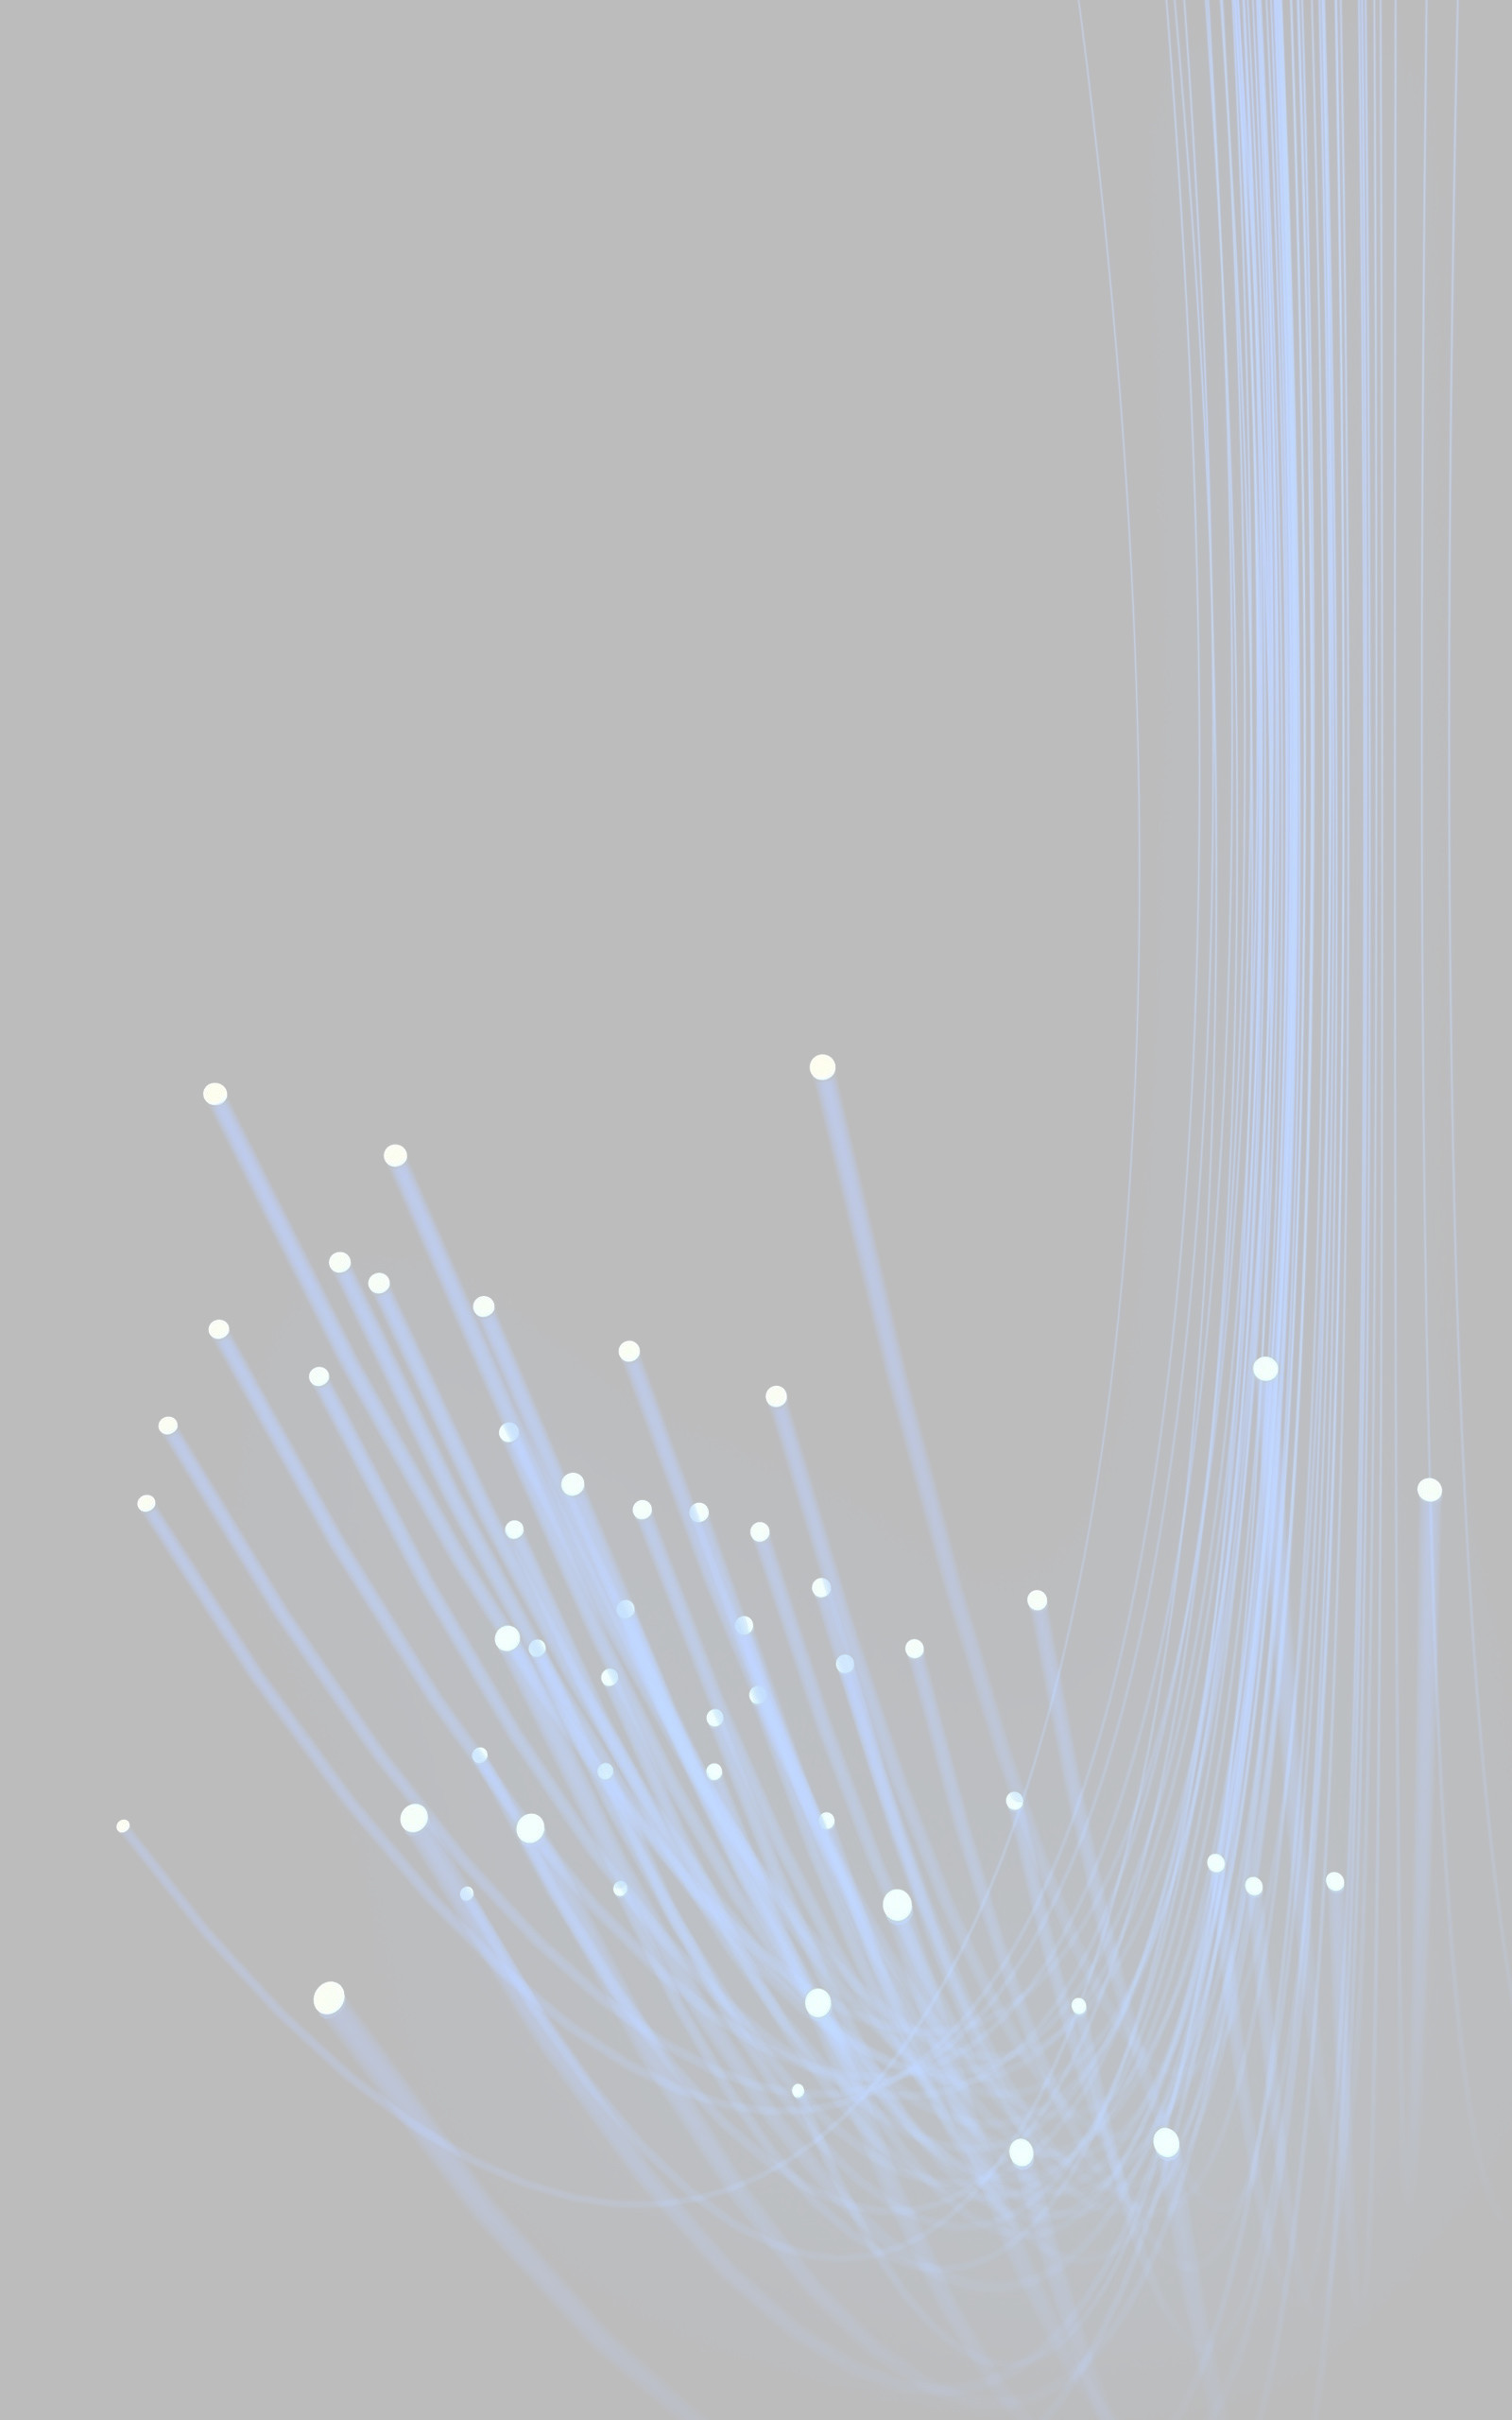
\includegraphics[scale=1]{capa}}} % Image background
	
	%\AddToShipoutPicture*{\put(116,650){
\includegraphics[scale=.75]{brasao.png}}} % Image background
	
	%\AddToShipoutPicture*{\put(244,200){
\includegraphics[scale=0.2]{ifgvertical}}} % Image background
	\AddToShipoutPicture*{\put(244,650){
\includegraphics[scale=0.2]{ifgvertical}}} % Image background
	
	\vspace*{4.5cm}
	
	\centering
	\par
	\fontsize{30}{30}
	\selectfont
	Algoritmos e Estruturas de Dados \\
	\vspace*{1.5cm}
	\par
	\fontsize{16}{16}
	\selectfont
	Tecnólogo em Análise e Desenvolvimento de Sistemas\\
	\vspace*{1.5cm}
	Prof. Dr. Waldeyr Mendes Cordeiro da Silva\\
	\vspace*{10cm}
	\par
	{\Huge 2019}
	\par
\endgroup
\pagebreak

%----------------------------------------------------------------------------------------
%	PEOPLE PAGE
%----------------------------------------------------------------------------------------
\chapterimage{banner3} % Chapter heading image
\par
\section*{Material didático para Algoritmos e Estruturas de Dados}

Versão 0.1

\section*{Autor: Waldeyr Mendes Cordeiro da Silva}\label{WaldeyrMendes}
\begin{itemize}
	\item Formação:
	\begin{itemize}
		\item Técnico em Processamento de Dados
		\item Bacharelado em Sistemas de Informação
		\item Licenciatura em Ciências Biológicas
		\item Complementação Pedagógica em Matemática
		\item Especialização em Engenharia de Software
		\item Especialização em Segurança da Informação
		\item Mestrado em Informática
		\item Doutorado em Ciências Biológicas (Bioinformática)
	\end{itemize}
	\item~~
\includegraphics[scale=.03]{Pictures/lattes}~~~\href{http://lattes.cnpq.br/2391349697609978}{Lattes: http://lattes.cnpq.br/2391349697609978}
	\item~~
\includegraphics[scale=.15]{Pictures/orcid}~~~\href{https://orcid.org/0000-0002-8660-6331}{ORCID: https://orcid.org/0000-0002-8660-6331}
	\item~
\includegraphics[scale=.05]{Pictures/scopus}~~~\href{https://www.scopus.com/authid/detail.uri?authorId=57190660358}{Scopus: https://www.scopus.com/authid/detail.uri?authorId=57190660358}
	\item 
\includegraphics[scale=.03]{Pictures/google}~\href{https://scholar.google.com.br/citations?user=5gh-liIAAAAJ}{Google Acadêmico: https://scholar.google.com.br/citations?user=5gh-liIAAAAJ}
\end{itemize}

\chapterimage{banner3} % Chapter heading image
\renewcommand\contentsname{Sumário}
\tableofcontents

%----------------------------------------------------------------------------------------
%	CHAPTER
%----------------------------------------------------------------------------------------
\chapterimage{01.jpg} % Chapter heading image
\chapter{Prefácio}\label{prefacio}
\vspace{6em}
\begin{flushright}
	\textit{\textcolor{white}{Um bonita citação...}}
\end{flushright}
\vspace{12em}

%\todo[inline]{Em construção...}

Este livro destina-se aos acadêmicos e demais interessados em iniciar os estudos em algoritmos e estruturas de dados.

%----------------------------------------------------------------------------------------
%	CHAPTER
%----------------------------------------------------------------------------------------
\chapterimage{02.jpg} % Chapter heading image
\chapter{Introdução}\label{introducao}
\vspace{6em}
\begin{flushright}
	\textit{\textcolor{white}{Um bonita citação...}}
\end{flushright}
\vspace{12em}

Um algoritmo é um procedimento computacional bem definido que processa um dado ou um conjunto de dados (entrada) e produz algum novo dado ou conjunto de dados (saída)~\cite{cormen2009}.
Os algoritmos existem há muito tempo, mas estão presentes na sociedade moderna de uma forma nunca experimentada nestes cerca de 2,5 milhões de anos da história humana.
Quase tudo que se produz, sejam produtos ou serviços, tem alguma influência de algoritmos.
O comércio eletrônico utiliza tanto algoritmos clássicos como ordenações, quanto algoritmos modernos de recomendação de produtos baseado no histórico de visitas.
A segurança das senhas em sistemas \textit{Web} ou bancários é baseada em algoritmos de criptografia.
Imagens de satélite, dados genômicos, reconhecimento de faces, previsão do tempo, quase tudo que se possa imaginar atualmente é influenciado direta ou indiretamente por algum algoritmo.

O estudo de algoritmos é uma demanda crescente frente aos novos desafios trazidos pelo grande volume de dados que as tecnologias modernas proporcionaram.
A análise de algortimos é uma área com questões importantes em aberto, como é o caso dos \textit{Millennium Prize Problems}, com sete problemas matemático-computacionais, cujo prêmio é de 1 milhão de dólares pela solução de cada problema.

\section{Análise de Algoritmos}\label{sec_analise}

O propósito da análise de um algortimo é prever seu comportamento quanto ao tempo de execução ou ao espaço em memória que irá ocupar mesmo antes de ser executado em um computador específico~\cite{manber1989}.
Muitos fatores, especialmente o tamanho e a variedade dos dos dados de entrada, influenciam o comportamento do algoritmo utilizando suas principais características.
Portanto, a análise de algoritmos provê uma aproximação, o que em muitos casos é bastante significante.
As possibilidades de entradas diferentes, ainda que de mesmo tamanho são muito vastas e por isso um algoritmos não se comportará da mesma maneira para diferentes entradas de um mesmo tamanho. 
Por esta razão a análise de algoritmos se concentra primordialmente em predizer o tempo aproximado de execução baseada no tamanho da entrada, tirando da equação elementos como o hardware, por exemplo.
Assim, ainda que haja uma variação no tempo de execução dependente da variabilidade da entrada, essa variação tem menor importância do que o tamanho da entrada.

Para entradas de tamanho ($n$) pequeno, qualquer algoritmo custa pouco para ser executado, portanto, a análise de algoritmos concentra-se em valores grandes de $n$~\cite{ziviani2007}.
O comportamento assintótico de uma função $f(n)$ representa o limite do comportamento do custo quando $n$ cresce.

\subsection{Elementos de Notação Assintótica}

\subsubsection{Notação Big O}
A notação $O$ denota um limite assintótico superior, ou seja, o pior caso, aquele que toma mais tempo de execução.
É importante ressaltar que existem notações para outros limites assintóticos, como médios ou inferiores.
Porém, aqui veremos a notação $O$,por ser uma das mais utilizadas para estimar o tempo de execução como limite superior.
Vejamos um exemplo. 
Tomando os valores $7, 2, 5, 4, 9$ dispostos desta maneira e lendo-os em ordem, encontraríamos o número $9$ em cinco passos.
Em outra entrada de mesmo tamanho, mas com os valores dispostos de outra maneira, $5, 9, 7, 4, 2$, encontraríamos o número $9$ em dois passos.
Independente das permutações possíveis, encontraríamos o número procurado em no máximo 5 passos, que é o pior caso, tomando entradas de mesmo tamanho e procurando desta exata maneira.

Na análise de algoritmos, as constantes, associadas ou não ao tamanho da entrada, têm baixa representatividade no tempo de execução~\cite{manber1989}.
Por exemplo, se um algoritmo executa em $2n^2+50$, dizemos que o algoritmo executa em $n^2$ pois as constantes $2$ e $50$ não interferem significativamente no crecismento assintótico da função.
O tempo de execução em função do tamanho da entrada está relacionado às várias classes de problemas que têm as seguintes funções de complexidade:
\begin{itemize}
\item $f(n) = O(1)~\mapsto$ Complexidade constante. O tempo de execução independe do tamanho ($n$) da entrada.
\item $f(n) = O(log~n)~\mapsto$ Complexidade logarítmica. Tempo de execução menor do que o de uma constante grande. Tipicamente são alcançados por algoritmos que dividem o problema em problemas menores.
\item $f(n) = O(n)~\mapsto$ Complexidade linear. Tempo de execução linear ao tamanho da entrada. São, em geral algoritmos que realizam pequenos trabalhos nos dados de entrada.
\item $f(n) = O(n~log~n)~\mapsto$ Essa complexidade ocorre normalmente em algoritmos que quebra o problema em partes menores, solucionam-as de forma independente juntando em seguida essas sub-soluções.
\item $f(n) = O(n^2)~\mapsto$ Complexidade quadrática. O crescimento quadrático significa que o tempo de execução crescerá rapidamente, pois será o quadrado do tamanho da entrada. Ou seja, para entradas grandes, o algoritmo levará muito tempo para ser executado.
\item $f(n) = O(n^3)~\mapsto$ Complexidade cúbica. Assim como o algoritmo de complexidade quadrática,  o tempo será o cubo do tamanho da entrada. Algoritmos desse tipo são úteis apenas para pequenas tarefas.
\item $f(n) = O(2^n)~\mapsto$ Complexidade exponencial. Algoritmos desse tipo geralmente não são úteis do ponto de vista prático. Geralmente são soluções baeadas em abordagens de ``força bruta''.
\item $f(n) = O(n!)~\mapsto$ Complexidade fatorial. São ainda piores em termos de tempo de execução do que os algoritmos exponenciais.
\end{itemize}

Geralmente não é uma tarefa trivial determinar se uma certa função $g(n)$ é $O(f(n))$.
Uma função $g(n)$ domina assintoticamente outra função $f(n)$ se existem constantes positivas $c$ e $n_0$ em que $n~\geq~n_0$ e $c.|g(n)|~\geq~|f(n)|$.
Ou seja, uma função é $O(g(n))$ se, para todos os valores de $n$ maiores que $n_0$, o valor da função $f(n)$ está abaixo de $g(n)$.
Para ilustrar melhor o domínio assintótico de uma função, considere as funções $g(n)=6n^2$ e $f(n) = 5n^2~+~15$, onde $n~\geq~4$. 
É possível ver que $g(n)~\geq~f(n)$ para $n~\geq~4$ na Figura~\ref{BigO}.

\begin{minipage}[c]{.5\textwidth}
\[ g(n) =
  \begin{cases}
    n=1  & 6.1^2 = 6\\
    n=2  & 6.2^2 = 24\\
    n=3  & 6.3^2 = 54\\
    n=4  & 6.4^2 = 96\\
    n=5  & 6.5^2 = 150\\
    n=6  & 6.6^2 = 216\\
    n=7  & 6.7^2 = 294\\
    ...
  \end{cases}
\]
\end{minipage}\hfill
\begin{minipage}[c]{.5\textwidth}
\[ f(n) =
  \begin{cases}
    n=1  & 5.1^2+15 = 20\\
    n=2  & 5.2^2+15 = 35\\
    n=3  & 5.3^2+15 = 60\\
    n=4  & 5.4^2+15 = 95\\
    n=5  & 5.5^2+15 = 140\\
    n=6  & 5.6^2+15 = 195\\
    n=7  & 5.7^2+15 = 260\\
    ...
  \end{cases}
\]
\end{minipage}
\hfill
\begin{figure}[htbp]
\centering
	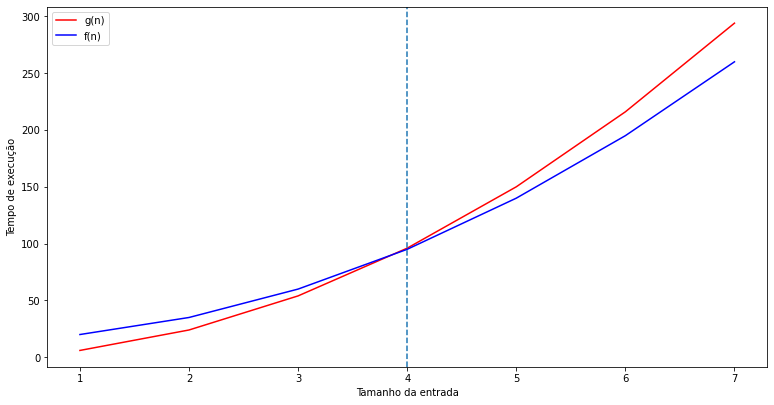
\includegraphics[width=.95\textwidth]{Pictures/BigO.png}
	\caption[Big O]{Domínio assintótico da função $g(n)$ sobre a função $f(n)$ quando $n~\geq~4$.}
	\label{BigO}
\end{figure}

Diz-se que uma função $f(n)$ cresce monotonamente se $n_1~\geq~n_2$, e portanto $f(n_1)~\geq~f(n_2)$.
Funções exponenciais crescem mais rápido do que funções polinomiais, ou seja, para as constantes $c~>~0$ e $a~> 1$, e para todas as funções $f(n)$ de crescimento monótono:
$$ (f(n))^c~=~O(a^f(n)) $$
Esta regra pode ser usada para comparar várias funções. Por exemplo, substituindo $f(n)$ por $n$ temos:
$$ n^c~=~O(a^n) $$
A Tabela~\ref{tab:garey1979} ilustra os tempos de execução para diferentes tamanhos de entrada em cada uma das complexidades exponenciais e polinomiais.
\begin{table}[htbp]
\centering
\caption{Comparação de tempos de execução polinomiais e exponenciais assumindo que 0,000001s é o tempo gasto para um $n = 1$. Adaptado de ~\textcite{garey1979}.}
\label{tab:garey1979}
\resizebox{\textwidth}{!}{%
\begin{tabular}{@{}lllllll@{}}
\toprule
\multirow{2}{*}{Complexidade} & \multicolumn{6}{l}{Tamanho da entrada (n)}                           \\ \cmidrule(l){2-7} 
                              & 10       & 20       & 30       & 40        & 50        & 60          \\ \midrule
$n$                           & 0,00001s & 0,00002s & 0,00003s & 0,00004s  & 0,00005s  & 0,00006s    \\ \midrule
$n^2$                         & 0,0001   & 0,0004s  & 0,0009s  & 0,0016s   & 0,0025s   & 0,0036s     \\ \midrule
$n^3$                         & 0,001s   & 0,008s   & 0,027s   & 0,064s    & 0,125s    & 0,216s      \\ \midrule
$2^n$                         & 0,001    & 1,0s     & 17,9 min & 12,7 dias & 35,7 anos & 366 séculos \\ \bottomrule
\end{tabular}%
}
\end{table}


%----------------------------------------------------------------------------------------
%	CHAPTER
%----------------------------------------------------------------------------------------
%------------------------------------------------
\chapterimage{04.jpg} % Chapter heading image
\chapter{Programação}\label{programacao}
\vspace{6em}
\begin{flushright}
	\textit{\textcolor{white}{Um bonita citação...}}
\end{flushright}
\vspace{12em}



\newpage
\section{Primeiros Passos em Programação}\label{disc:primeirospassos}

Dennis Ritchie criou a linguagem ``C'' em 1972 quando trabalhava nos laboratórios da Bell Telephone.
A linguagem C foi criada para desenvolver uma nova versão do sistema operacional Unix que utilizava Assembly até então.
Inicialmente, a cada nova implementação de Unix para um tipo de máquina, um novo compilador C devia ser desenvolvido para essa máquina.
Nos anos 80, C tornou-se popular fora do ambiente Unix, criando a demanda por compiladores comerciais.
Desde então, C é considerada uma linguagem de propósito geral, com instruções de alto nível e capaz de gerar programas rápidos em tempo de execução.
Além disso, C influenciou de forma direta a sintaxe e estruturas de linguagens modernas como C++, Java, C\#, Objective C, e muitas outras.

A linguagem C começou a ser padronizada pela \textit{American National Standards Institute} (ANSI) para garantir a compatibilidade e a portabilidade da linguagem.
Este padrão foi atualizado ao longo do tempo e posteriormente reconhecido pela ISO, dando origem ao padrão ANSI/ISO.

Um código escrito em linguagem C funciona com comandos, que são normalmente palavras em inglês (sintaxe) e são organizados em determinadas estruturas.
Uma vez escritos em um arquivo, os comandos são então lidos pelos compiladores e convertidos para a linguagem de máquina que corresponde a ação pretendida.
O Programa~\ref{prog001} mostra um exemplo de programa em C.

\lstinputlisting[label={prog001},language=C, caption={Meu primeiro programa em C.}]{Code/Basics/prog001.c}

Após escrito, o programa precisa ser compilado. 
Se o programa tiver sido escrito corretamente (sintaxe e estrutura), o compilador gera um executável.
É importante peceber, que compiladores não verificam erros lógicos, ou seja de concepção do código.
É justamente aí que reside o valor do trabalho humano como programador: combinar sintaxe e estruturas de forma que solucionem um dado problema do mundo real.
Caso o compilador encontre algum erro no código dois tipos de mensagens podem ser emitidas:
\begin{enumerate}
	\item Erro (\textit{error}): Quando o código tem um problema que impede o compilador de gerar um executável
	\item Aviso (\textit{warnning}): Quando o problema no código não impede de gerar um executável, mas requer algum tipo de atenção.
\end{enumerate}

Para compilar o Programa~\ref{prog001} em Linux com o compilador C (Veja aqui como instalar) basta o seguinte comando no terminal: 
\terminal{gcc prog001.c -o prog001.sh}

Após esta ação, será gerado o arquivo executável \texttt{prog001.sh}, o qual poderá ser executado com o comando: 
\terminal{./prog001.sh}

No Programa~\ref{prog001} é impressa uma mensagem na tela. 
O catacter especial representado por ``$\backslash$n'' identifica uma quebra de linha.
Essa mensagem é representada como uma cadeira de caracteres (\textit{string}) limitada pelas aspas.
Se for necessário representar as aspas em uma \textit{string}, será necessário escapá-las usando a barra ``$\backslash$''.
O Programa~\ref{prog002} mostra como fazer isso.

\lstinputlisting[label={prog002},language=C, caption={Escapando aspas.}]{Code/Basics/prog002.c}

\section{Trabalhando com Variáveis}

Uma variável é um objeto capaz de guardar e representar um valor ou expressão em memória. 
Às variáveis são associadas a nomes ou identificadores e sua existência é limitada por um espaço e um tempo na memória do computador, o qual frequentemente é igual ao tempo de execução do programa em que elas foram criadas.

Nas linguagen de programação é comum existirem tipos de dados pré-definidos, chamados tipo primitivos.
Em C, os tipo primitivos são:

\begin{itemize}
	\item char: caracter
	\item int: inteiro
	\item float: real de precisão simples
	\item double: real de alta precisão
	\item void: vazio ou sem valor
\end{itemize}

Há ainda os modificadores que alteram o tamanho, e consequentemente sua capacidade, dos tipos em memória. São eles:

\begin{itemize}
	\item signed
	\item unsigned
	\item long
	\item short
\end{itemize}

Combinando os tipo e os modificadores temos:

\begin{table}[htbp]
	\centering
	\caption{}
	\label{tab:tipos_modificadores}
	\resizebox{\textwidth}{!}{%
		\begin{tabular}{@{}llcr@{}}
			\toprule
			\multicolumn{1}{c}{Palavra chave} & \multicolumn{1}{c}{Tipo}                 & Tamanho (Bytes) & \multicolumn{1}{c}{Intervalo}  \\ \midrule
			char                              & Caracter                                 & 1       & -128 a 127                     \\
			signed char                       & Caractere com sinal                      & 1       & -128 a 127                     \\
			unsigned char                     & Caractere sem sinal                      & 1       & 0 a 255                        \\
			int                               & Inteiro                                  & 4       & -32.768 a 32.767               \\
			signed int                        & Inteiro com sinal                        & 4       & -32.768 a 32.767               \\
			unsigned int                      & Inteiro sem sinal                        & 4       & 0 a 65.535                     \\
			short int                         & Inteiro curto                            & 2       & -32.768 a 32 767               \\
			signed short int                  & Inteiro curto com sinal                  & 2       & -32.768 a 32.767               \\
			unsigned short int                & Inteiro curto sem sinal                  & 2       & 0 a 65.535                     \\
			long int                          & Inteiro long                             & 8       & -2.147.483.648 a 2.147.483.647 \\
			signed long int                   & Inteiro longo com sinal                  & 8       & -2.147.483.648 a 2.147.483.647 \\
			unsigned long int                 & Inteiro longo sem sinal                  & 8       & 0 a 4.294.967.295              \\
			float                             & Ponto flutuante com precisão simples     & 4       & 3.4 E-38 a 3.4E+38             \\
			double                            & Ponto flutuante com precisão simples     & 8       & 1.7 E-308 a 1.7E+308           \\
			long double                       & Ponto flutuante com precisão dupla longo & 16      & 3.4E-4932 a 1.1E+4932          \\ \bottomrule
		\end{tabular}%
	}
\end{table}

O Programa~\ref{prog003} mostra um exemplo de variável representando o valor inteiro 10 e em seguida a impressão de uma mensagem com seu valor.
Na impressão, é importante notar que a mensagem é formatada para que em um dterminado ponto ($\backslash$d) apareçam os dígitos correspondentes ao valor de \texttt{a} que é a variável abrigando o valor 10.

\lstinputlisting[label={prog003},language=C, caption={Trabalhando com variáveis.}]{Code/Basics/prog003.c}

As formas de declarrar variáveis podem ser diversas. O Programa~\ref{prog004} mostra a delaração de variáveis $n1$ e $n2$ atribuindo imediatamente os valores, enquanto a vairiável $soma$ é criada sem que seu valor seja atribuído imediatamente. No Programa~\ref{prog005}, as variáveis $n1$ e $n2$ são declaradas na mesma linha, separadas por vírgula, uma vez que são do mesmo tipo $int$.

\lstinputlisting[label={prog004},language=C, caption={Trabalhando com variáveis.}]{Code/Basics/prog004.c}

\lstinputlisting[label={prog005},language=C, caption={Trabalhando com variáveis.}]{Code/Basics/prog005.c}

Quanto à atribuição de valores à uma variável, ela pode ser direta ou indireta, ou seja, um valor pode ser diretamente atribuído à uma variável ou o valor de uma variável pode ser atribuído a outra, como no exemplo do Programa~\ref{prog006}, onde $n1$ recebe o valor de $n2$ que recebe o valore de $n3$ que recebe $10$. Nesse caso, $n1$, $n2$ e $n3$ terão valor = $10$.

\lstinputlisting[label={prog006},language=C, caption={Trabalhando com variáveis.}]{Code/Basics/prog006.c}

Dependendo do tipo primitivo de dados da variável, diferentes formatações podem ser usadas paara a função printf() conforme pode ser visto na Tabela~\ref{tab:printf}. O Programa~\ref{prog007} ilustra um exemplo de impressão de um float com 2 casa decimais.

\lstinputlisting[label={prog007},language=C, caption={Trabalhando com variáveis.}]{Code/Basics/prog007.c}


\begin{table}[ht]
	\centering
	\caption{Formatação da saída de dados com a função printf().}
	\label{tab:printf}
		\begin{tabular}{@{}ll@{}}
			\toprule
			Formatação & Significado                        \\ \midrule
			\%c        & caracter                           \\
			\%d        & inteiro  base 10                   \\
			\%e        & exponencial ponto flutuante        \\
			\%f        & ponto flutuante                    \\
			\%i        & integer (base 10)                  \\
			\%o        & octal (base 8)                     \\
			\%s        & \textit{string}                    \\
			\%u        & \textit{unsigned} inteiro          \\
			\%x        & hexadecimal (base 16)              \\
			\%\%       & caracter de porcentagem            \\ \bottomrule
		\end{tabular}%
\end{table}

O Programa~\ref{prog008}  mostra algumas variáveis e seus respectivos tamanhos em \textit{Bytes} com sua saída formatada.

\lstinputlisting[label={prog008},language=C, caption={Trabalhando com variáveis.}]{Code/Basics/prog008.c}

\subsubsection{Operadores Aritméticos}

Os operadores aritméticos usados em C são mostrados na Tabela~\ref{tab:opareadores_aritmeticos}.
\begin{table}[htbp]
	\centering
	\caption{Operadores aritméticos.}
	\label{tab:opareadores_aritmeticos}
		\begin{tabular}{@{}ll@{}}
			\toprule
			\textbf{Operador}             & \textbf{Sintaxe} \\ \midrule
			Adição unária                 & +a               \\
			Adição                        & a + b            \\
			Incremento pré-fixado         & ++a              \\
			Incremento pós-fixado         & a++              \\
			Atribuição por adição         & a += b           \\
			Subtração unária              & -a               \\
			Subtração                     & a - b            \\
			Decremento pré-fixado         & --a              \\
			Decremento pós-fixado         & a--              \\
			Atribuição por subtração      & a -= b           \\
			Multiplicação                 & a * b            \\
			Atribuição por multiplicação  & a *= b           \\
			Divisão                       & a / b            \\
			Atribuição por divisão        & a /= b           \\
			Módulo (resto)                & a \% b           \\
			Atribuição por módulo (resto) & a \%= b          \\ \bottomrule
		\end{tabular}%
\end{table}
\begin{table}[htb]
	\centering
	\caption{Precedência de operadores.}
	\label{tab:prioridade_operadores}
		\begin{tabular}{@{}ll@{}}
			\toprule
			\textbf{Prioridade} & \textbf{Operadores}                                                                \\ \midrule
			1º                  & Parênteses internos                                                                \\
			2º                  & potência (\textasciicircum{}) e raiz (quando a linguagem oferece esses operadores) \\
			3º                  & * / div e mod                                                                      \\
			4º                  & + e -                                                                              \\ \bottomrule
		\end{tabular}%
\end{table}
O Programa~\ref{prog009} ilustra o uso do operador \textit{mod}, que retorna o resto da divisão inteira.
\lstinputlisting[label={prog009},language=C, caption={Trabalhando com variáveis.}]{Code/Basics/prog009.c}

\subsubsection{Entrada de Dados}

A maneira mais clássica de um programa em C obter dados digitados pelo o usuário através do \textit{prompt} é usando a função \textit{scanf()}. 
O Programa~\ref{prog010} mostra um exemplo onde os valores das variáveis $a$ e $b$ são informados pelo usuário e depois somados.
\lstinputlisting[label={prog010},language=C, caption={Trabalhando com a função \textit{scanf()} para entrada de dados em C.}]{Code/Basics/prog010.c}

\section{Estruturas de Decisão}

\subsection{If/Else}

O \textit{if} é utilizado para testar uma proposição lógica.
A proposição é escrita entre parênteses.
Caso o resultado seja verdadeiro, o bloco de instruções subordinadas ao \textit{if} será executado.
O bloco é delimitado por ``\{'' e ``\}''. 
Se houver apenas uma instrução subordinada, não há necessidade das chaves.

O \textit{else} é utilizado para capturar a condição não atendida no teste do \textit{if}, o ``caso contrário''.
O Programa~\ref{prog011} mostra um exemplo onde o valor da variável $x$ é testado para saber se é maior ou igual a zero.
Através deste teste é possível identificar se o valor é positivo (\textit{if} verdadeiro $\rightarrow valor >= 0 $), ou é negativo (\textit{else} $\rightarrow valor < 0$).
\lstinputlisting[label={prog011},language=C, caption={Trabalhando com o \textit{if} em C.}]{Code/Basics/prog011.c}

Há ainda a possibilidade verificar múltiplas condições com o \textit{else if}.
O uso do \textit{else if} é demonstrado no Programa~\ref{prog012} que verifica se um valor inteiro informado pelo usuário é = 10, 20 ou 30.
\lstinputlisting[label={prog012},language=C, caption={Trabalhando com o \textit{if, else if, else} em C.}]{Code/Basics/prog012.c}

Um exemplo onde caracteres podem ser usados é mostrado no Programa~\ref{prog013}.
Neste programa uma questão apresenta alternativas $a$, $b$, $c$, $d$ e $e$. 
O usuário escolhe a letra correspondente à resposta corrta e o programa diz se ele acertou ou não. 
Além disso, reporta se a opção escolhida é inválida.
\lstinputlisting[label={prog013},language=C, caption={Trabalhando com o \textit{if, else if, else} em C.}]{Code/Basics/prog013.c}

%----------------------------------------------------------------------------------------
%	CHAPTER X
%----------------------------------------------------------------------------------------
%------------------------------------------------
\chapterimage{05.jpg} % Chapter heading image
\chapter{Estruturas de Dados}\label{estrutura}
\vspace{6em}
\begin{flushright}
	\textit{\textcolor{white}{Um bonita citação...}}
\end{flushright}
\vspace{12em}

Tipos abstratos de dados são conjuntos de valores sobre os quais é possível aplicar funções de forma homogênea através de um algortimo.
Funções e valores em conjunto, consituem um modelo matemático que pode ser empregado em problemas do mundo real~\cite{ascencio2010}.
Os algortimos são projetados em função de um tipo abstrato de dados.
A representação computacional de um tipo abstrato de dados com seus tipos e operações permitidas pode ser entendida como uma \textbf{estrutura de dados}.
Uma estrutura de dados é um meio para armazenar e processar dados com vistas à sua organização, acesso e modificações~\cite{cormen2009}.


\newpage
\section{Estruturas de Dados Homogêneas e Heterogêneas}\label{tipos}

\subsection*{Vetores}

Primeiro, uma revisão sobre vetores.
Em C uma variável que represente um vetor é um ponteiro.
Portanto, quando um vetor é parâmetro para uma função o que é passado é a sua referência, ou seja, o endereço base do vetor.
Vetores podem ser bi-, tri-, ou multi-domensionais, mas abrigam o mesmo tipo de dados.
O programa~\ref{rev001} mostra o vetor sendo passado para uma função que retorna o valor do meio do vetor.

\lstinputlisting[language=C, caption={Em C, vetores são passados para funções por referência.}]{Code/Revisao/rev001.c}\label{rev001}

\lstinputlisting[language=C, caption={Um vetor de duas dimensões mostrando apenas valores da diagonal principal.}]{Code/Revisao/rev003.c}\label{rev003}

\subsection*{Strings em C}
Em C, uma \textit{string} é um vetor de caracteres e cada \textit{string} termina com um caracter \textit{NULL}.
Uma constante \textit{string} é definida dentro de aspas em que o caractere \textit{NULL} é automaticamente incluído.
Por exemplo, a string "IFG" é um vetor de 4 elementos.
O programa~\ref{rev002} mostra um exemplo de \textit{string} em C. 
\lstinputlisting[language=C, caption={Em C, \textit{strings} são vetores de caracteres..}]{Code/Revisao/rev002.c}\label{rev002}


\subsection*{Structs}
Em C, uma \textit{struct} é uma forma de criar novos tipos heterogêneos.
O programa~\ref{struct01} mostra um exemplo de \textit{struct} em C. 

\newpage
\lstinputlisting[language=C, caption={Structs em C.}]{Code/Listas/Struct.c}\label{struct01}

\newpage
O programa~\ref{struct02} mostra um exemplo de composição de \textit{struct} em C. 
\lstinputlisting[language=C, caption={Composição de Structs em C.}]{Code/Listas/Struct2.c}\label{struct02}

\section{Listas Encadeadas}

Uma lista encadeada é uma estrutura de dados que permite um crescimento sob demanda, limitado à capacidade de memória disponível no computador.
Ela é composta de ``nós'' que tem suas posições de memória ligadas através de ponteiros. 
Cada nó da lista, além de guardar dados em si, aponta o próximo nó.
Os dados em um nó também podem ser heterogêneos.
A Figura~\ref{listaEncadeada} ilustra essa ideia. 
Apesar da figura dar a impressão de que os nós estão distribuídos contiguamente na memória, eles estão na verdade espalhados em endereços aleatórios de memória. 
Por isso o encadeamento funciona com ponteiros apontando o endereço de memória do próximonó da lista.
\begin{figure}
	\centering
	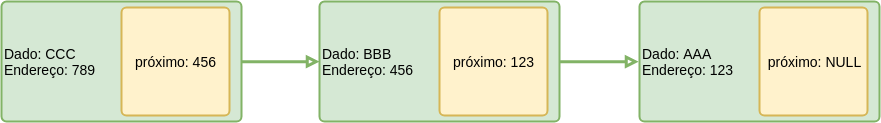
\includegraphics[width=.7\textwidth]{Pictures/ListaEncadeada01.png}
	\caption[Lista Encadeada]{Representação de uma Lista Encadeada.}
	\label{listaEncadeada}
\end{figure}
O  programa~\ref{ListaEncadeada01} apresenta uma implementação em C de uma lista encadeada.
\newpage
\lstinputlisting[language=C, caption={Implementação em C de lista encadeada.}]{Code/Listas/ListaEncadeada02.c}\label{ListaEncadeada01}

\newpage
As listas encadeadas podem conter ponteiros para outro nós além do próximo. 
É possível criar uma lista com \textit{links} simultâneos para o próximo nó e para o nó anterior.
Essas listas são conhecidas como listas duplamente encadeadas.
O  programa~\ref{ListaEncadeada03} apresenta uma implementação em C de uma duplamente encadeada.

\lstinputlisting[language=C, caption={Implementação em C de lista duplamente encadeada.}]{Code/Listas/ListaEncadeada03.c}\label{ListaEncadeada03}

\section{Pilhas}\label{pilhas}

\section{Filas}\label{filas}

\section{Algoritmos de Ordenação}\label{ordenacao}

\subsection*{Bubble Sort}
O algoritmo da bolha (\textit{Bubble Sort}) é um algortimo de ordenação onde cada elemento de uma posição $i$ é comparado com o elemento de posição $i+1$, os quais trocam de posição, se for o caso, para atender à ordenação procurada (crescente ou decrescente).
O  programa~\ref{BubbleSort} apresenta uma implementação em C do algoritmo \textit{Bubble Sort}, enquanto a Figura~\ref{diaBubleSort} ilustra seu funcionamento para um vetor de tamanho 4.
\lstinputlisting[language=C, caption={Implementação em C do algoritmo de ordenação BubbleSort.}]{Code/Ordenacao/BubbleSort.c}\label{BubbleSort}
\begin{figure}
	\centering
	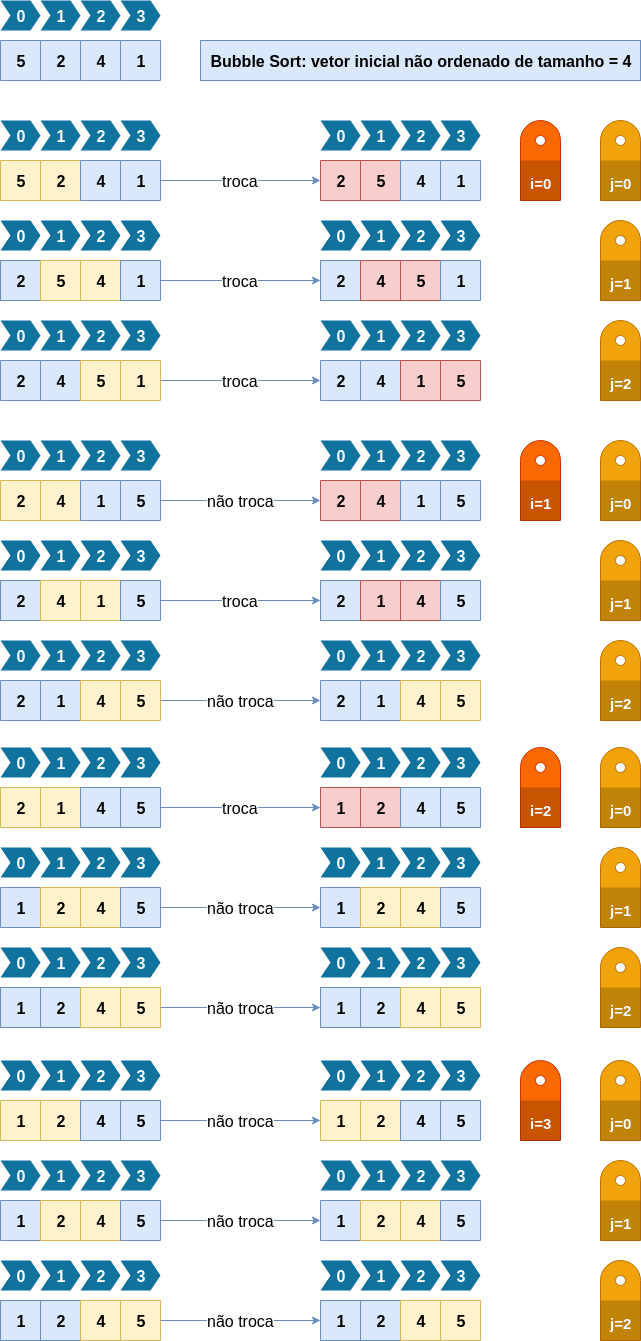
\includegraphics[width=.7\textwidth]{Pictures/BubbleSort}
	\caption[Bubble Sort]{Algoritmo \textit{Bubble Sort} para um vetor de tamanho 4.}
	\label{diaBubleSort}
\end{figure}

\subsection*{Exercícios}
\begin{enumerate}
	\item Atualizar a implementação do \textit{Bubble Sort} para executar as seguinte tarefa:
	\begin{itemize}
		\item executar o algoritmo com três vetores de entrada:
		\begin{enumerate}
			\item um vetor ordenado crescente de tamanho 100000 (cem mil)
			\item um vetor com números aleatórios de tamanho 100000 (cem mil)
			\item um vetor ordenado decrescente de tamanho 100000 (cem mil)
		\end{enumerate} 
		\item criar variáveis para contar a quantidade de comparações e quantidade de trocas;
	\end{itemize} 
	\item Criar gráficos para as três execuções comparando quantidade de comparações e quantidade de trocas e o tempo de execução;
\end{enumerate} 

\newpage
\subsection*{Selection Sort}
No algoritmo de ordenação por seleção (\textit{Selection Sort}) cada número do vetor, a partir do primeiro, é eleito e comparado com o menor número\footnote{Ou maior dependendo da ordenação desejada.} entre aqueles que estão à direita do eleito.
O  programa~\ref{SelectionSort} apresenta uma implementação em C do algoritmo \textit{Selection Sort} para um vetor de tamanho 4.
%, e a Figura~\ref{diaSelectionSort} ilustra seu funcionamento.
\lstinputlisting[language=C, caption={Implementação em C do algoritmo de ordenação Selection.}]{Code/Ordenacao/SelectionSort.c}\label{SelectionSort}
%\begin{figure}
%	\centering
%	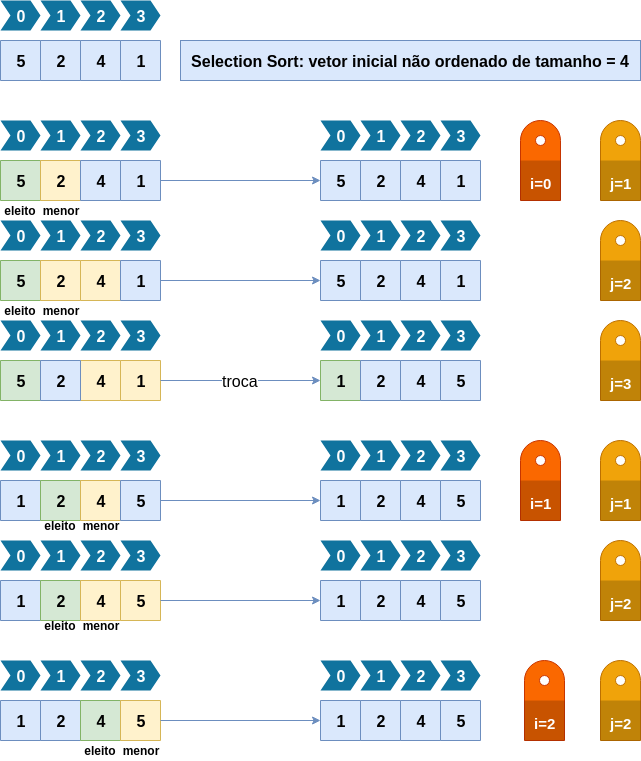
\includegraphics[width=.75\textwidth]{Pictures/SelectionSort}
%	\caption[Selection Sort]{Algoritmo \textit{Selection Sort} para um vetor de tamanho 4.}
%	\label{diaSelectionSort}
%\end{figure}

\subsection*{Exercícios}
\begin{enumerate}
	\item Atualizar a implementação do \textit{Selection Sort} para executar as seguinte tarefa:
	\begin{itemize}
		\item executar o algoritmo com três vetores de entrada:
		\begin{enumerate}
			\item um vetor ordenado crescente de tamanho 100000 (cem mil)
			\item um vetor com números aleatórios de tamanho 100000 (cem mil)
			\item um vetor ordenado decrescente de tamanho 100000 (cem mil)
		\end{enumerate} 
		\item criar variáveis para contar a quantidade de comparações e quantidade de trocas;
	\end{itemize} 
	\item Criar gráficos para as três execuções comparando quantidade de comparações e quantidade de trocas e o tempo de execução;
\end{enumerate} 
\newpage
\subsection*{Insertion Sort}
O algoritmo de ordenação por inserção (\textit{Insertion Sort}), funciona como uma mão de baralho onde você ordena suas cartas começando a comparação entre as duas primeiras.
No \textit{Insertion Sort}, é eleito o segundo elemento do vetor para iniciar a comparção. É percorrido o vetor de forma a garantir que todos os números à esquerda do eleito sejam menores que ele.
O programa~\ref{InsertionSort} apresenta uma implementação em C do algoritmo \textit{Insertion Sort} para um vetor de tamanho 4.
\lstinputlisting[language=C, caption={Implementação em C do algoritmo de ordenação Insertion Sort.}]{Code/Ordenacao/InsertionSort.c}\label{InsertionSort}
%\begin{figure}
%	\centering
%	\includegraphics[width=.75\textwidth]{Pictures/InsertionSort}
%	\caption[Selection Sort]{Algoritmo \textit{Selection Sort} para um vetor de tamanho 4.}
%	\label{diaInsertionSort}
%\end{figure}

\subsection*{Exercícios}
\begin{enumerate}
	\item Atualizar a implementação do \textit{Insertion Sort} para executar as seguinte tarefa:
	\begin{itemize}
		\item executar o algoritmo com três vetores de entrada:
		\begin{enumerate}
			\item um vetor ordenado crescente de tamanho 100000 (cem mil)
			\item um vetor com números aleatórios de tamanho 100000 (cem mil)
			\item um vetor ordenado decrescente de tamanho 100000 (cem mil)
		\end{enumerate} 
		\item criar variáveis para contar a quantidade de comparações e quantidade de trocas;
	\end{itemize} 
	\item Criar gráficos para as três execuções comparando quantidade de comparações e quantidade de trocas e o tempo de execução;
\end{enumerate} 
\newpage
\subsection*{Merge Sort}
O algoritmo de ordenação \textit{Merge Sort} a técnica de divisão e conquista, ou seja, o problema é dividido em subproblemas menores até que a solução para o subproblema seja simples.
As soluções dos subproblemas são combinadas para prover a solução do problema original.

No \textit{Merge Sort}, o vetor é dividido em partes iguais recursivamente até que haja apenas um elemento. Por exemplo se um vetor tem $n$ elementos, ele é divido em $n/2$, o resultado é novamente dividido por $2$ até que o vetor não seja mais divisível.
Os pares da última divisão são ordenados entre si assim como na volta recursiva montando o vetor original que estará então ordenado.
O programa~\ref{MergeSort} apresenta uma implementação em C do algoritmo \textit{Merge Sort} para um vetor de tamanho 4.
\lstinputlisting[language=C, caption={Implementação em C do algoritmo de ordenação Merge Sort.}]{Code/Ordenacao/MergeSort.c}\label{MergeSort}

\subsection*{Exercícios}
\begin{enumerate}
	\item Atualizar a implementação do \textit{Merge Sort} para executar as seguinte tarefa:
	\begin{itemize}
		\item executar o algoritmo com três vetores de entrada:
		\begin{enumerate}
			\item um vetor ordenado crescente de tamanho 100000 (cem mil)
			\item um vetor com números aleatórios de tamanho 100000 (cem mil)
			\item um vetor ordenado decrescente de tamanho 100000 (cem mil)
		\end{enumerate} 
		\item criar variáveis para contar a quantidade de comparações e quantidade de trocas;
	\end{itemize} 
	\item Criar gráficos para as três execuções comparando quantidade de comparações e quantidade de trocas e o tempo de execução;
\end{enumerate} 


\newpage
\subsection*{Quick Sort}
O algoritmo de ordenação \textit{Quick Sort} também utiliza a técnica de divisão e conquista.
No \textit{Quick Sort}, o vetor é dividido em duas partes recursivamente a partir de um pivô escolhido, até que não seja possível dividir mais. 
Os pares da última divisão são ordenados entre si assim na volta recursiva colocando todos os valores menores que o pivô no vetor à sua esquerda e todos os valores maiores que o pivô no vetor à sua direita.
Após esse procedimento o pivô estará ordenado em sua posição com relação os demais números.
O programa~\ref{QuickSort} apresenta uma implementação em C do algoritmo \textit{Quick Sort} para um vetor de tamanho 4.
\lstinputlisting[language=C, caption={Implementação em C do algoritmo de ordenação Quick Sort.}]{Code/Ordenacao/QuickSort.c}\label{QuickSort}

\subsection*{Exercícios}
\begin{enumerate}
	\item Atualizar a implementação do \textit{Quick Sort} para executar as seguinte tarefa:
	\begin{itemize}
		\item executar o algoritmo com três vetores de entrada:
		\begin{enumerate}
			\item um vetor ordenado crescente de tamanho 100000 (cem mil)
			\item um vetor com números aleatórios de tamanho 100000 (cem mil)
			\item um vetor ordenado decrescente de tamanho 100000 (cem mil)
		\end{enumerate} 
		\item criar variáveis para contar a quantidade de comparações e quantidade de trocas;
	\end{itemize} 
	\item Criar gráficos para as três execuções comparando quantidade de comparações e quantidade de trocas e o tempo de execução;
\end{enumerate} 

\newpage
\section{Árvores}\label{arvores}

O  programa~\ref{ArvoreBinaria01} apresenta uma implementação em C de uma árvore binária.
A representação gráfica da árvore é feita usando a biblioteca \href{http://graphviz.org/}{Graphviz}~\cite{Ellson03graphvizand}.

\lstinputlisting[language=C, caption={Implementação em C de lista duplamente encadeada.}]{Code/ArvoreBinaria/ArvoreBinaria.c}\label{ArvoreBinaria01}

\section{Tabelas Hashing}\label{hashing}

\section{Grafos}\label{grafos}

\subsection{Busca em Grafos}

%----------------------------------------------------------------------------------------
%	CHAPTER X
%----------------------------------------------------------------------------------------
%------------------------------------------------
\chapterimage{06.jpg} % Chapter heading image
\chapter{Aplicações}\label{aplicacoes}
\vspace{6em}
\begin{flushright}
	\textit{\textcolor{white}{Um bonita citação...}}
\end{flushright}
\vspace{12em}


% ----------------------------------------------------------------------------------------
% 	BIBLIOGRAPHY
% ----------------------------------------------------------------------------------------
%----------------------------------------------------------------------------------------
%	CHAPTER X
%----------------------------------------------------------------------------------------
%------------------------------------------------
\chapterimage{07.jpg} % Chapter heading image
%\chapter*{Referências Bibliográficas}
%\bibliography{bibliography}
%\renewcommand\bibname{Referências Bibliográficas}

\chapter*{Referências Bibliográficas}\label{referencias}
\vspace{6em}
\begin{flushright}
	\textit{\textcolor{white}{Um bonita citação...}}
\end{flushright}
\vspace{12em}
%\addcontentsline{toc}{chapter}{\textcolor{verde}{Bibliography}}
%\section{Books}
%\addcontentsline{toc}{section}{Books}
%\printbibliography[heading=bibempty,type=book]
%\section{Articles}
%\addcontentsline{toc}{section}{Articles}
%\printbibliography[heading=bibempty,type=article]
\printbibliography[heading=bibempty]


%----------------------------------------------------------------------------------------

%----------------------------------------------------------------------------------------
%	INDEX
%----------------------------------------------------------------------------------------
%
%\cleardoublepage
%\phantomsection
%\setlength{\columnsep}{0.75cm}
%\addcontentsline{toc}{chapter}{\textcolor{verde}{Index}}
%\printindex


%----------------------------------------------------------------------------------------
%	CHAPTER X
%----------------------------------------------------------------------------------------
%------------------------------------------------
\chapterimage{08.jpg} % Chapter heading image
\chapter{Apêncice}\label{apendice}
\vspace{6em}
\begin{flushright}
	\textit{\textcolor{white}{}}
\end{flushright}
\vspace{12em}


\end{document}
